\section{问题一:确定性环境下的多周期优化模型}

问题一旨在为该乡村规划2024年至2030年共七年的农作物种植策略。该问题本质上是一个在完全信息假设下的多周期资源分配问题。从微观经济学视角看,这相当于将该乡村抽象为一个理性的经济主体,其在拥有固定的生产技术、资源禀赋和已知的市场参数条件下,追求长期利润的最大化。由于决策变量中既包含连续的种植面积,也包含是否种植的离散选择,该问题能够被精确地构建为一个大规模的多周期混合整数线性规划(MILP)模型。本章将详细阐述该模型的构建、求解与分析过程,旨在为后续更复杂的分析提供一个确定性环境下的最优基准。

模型的顶层设计如图\ref{fig:milp_framework}所示,它清晰地展示了模型的输入、处理核心与输出。该框架整合了土地资源、作物属性、经济参数和农艺规则,通过MILP求解器进行优化,最终生成最优的七年种植方案与相应的经济效益预测。

% \begin{figure}[htbp]
%     \centering
%     \includegraphics[width=0.8\textwidth]{figures/milp_framework.png}
%     \caption{问题一的混合整数线性规划模型概念框架图。该框架整合了多源输入数据,通过优化核心生成最优种植方案与经济预测,为确定性环境下的决策提供了系统性方法。}
%     \label{fig:milp_framework}
% \end{figure}

\subsection{模型构建}


为将该乡村的长期种植规划问题转化为一个可求解的数学模型,我们构建了一个多周期混合整数线性规划(MILP)模型。该模型以古典微观经济学中的厂商理论为基础,将乡村视为一个追求长期利润最大化的理性决策主体。模型的构建过程遵循模块化原则,依次定义了决策变量、目标函数和约束条件三个核心部分。

\subsubsection{决策变量}

模型的决策核心在于如何在给定的时间和空间维度上分配种植资源。为此,我们定义了以下三组核心决策变量,它们共同构成了完整的七年种植方案:
\begin{itemize}
	\item \textbf{种植面积变量 ($x_{ijky}$)}: 这是一个连续变量,代表在年份 $y \in Y$ 的季节 $k \in K$,于地块 $i \in I$ 安排种植作物 $j \in J$ 的具体面积。该变量是模型的核心,直接关联到成本与产出。
	\item \textbf{种植决策变量 ($u_{ijky}$)}: 这是一个二进制变量,用于表征种植行为的有无。当且仅当在地块 $i$ 的 $y$ 年 $k$ 季实际安排了作物 $j$ 的种植(即 $x_{ijky} > 0$)时,$u_{ijky}$ 取值为1,否则为0。该变量主要用于处理与规模化经营相关的逻辑约束。
	\item \textbf{年度种植状态变量 ($z_{ijy}$)}: 这是一个年度层面的二进制变量。若在年份 $y$ 的任何一个季节,地块 $i$ 安排了作物 $j$ 的种植,则 $z_{ijy}$ 取值为1,否则为0。该变量用于聚合季节性种植信息,以简化跨年度农艺约束的表达。
\end{itemize}
此外,为处理产出与销售环节的逻辑,引入了两组关键的辅助变量:
\begin{itemize}
	\item \textbf{正常销售量 ($Sales_{jky}$)}: 表示作物 $j$ 在年份 $y$ 季节 $k$ 的总产量中,在预期市场需求内,按正常市场价格销售的数量。
	\item \textbf{超产销售量 ($OverSales_{jky}$)}: 表示作物 $j$ 在年份 $y$ 季节 $k$ 的总产量中,超出预期市场需求后,进行降价处理的销售数量。
\end{itemize}

\subsubsection{目标函数}

模型的目标是最大化在整个七年规划期(2024-2030)内的累计净利润。根据题目设定的两种不同市场情景,分别构建对应的目标函数。

\textbf{情景一:超产滞销}

在此情景下,任何超出市场预期需求量的产量均无法转化为经济收益,其价值为零。因此,总收益仅由正常销售部分贡献。目标函数定义为:
\begin{equation}
	\max \sum_{y \in Y} \sum_{k \in K} \left( \sum_{j \in J} P_j \cdot Sales_{jky} - \sum_{j \in J} \sum_{i \in I} C_j \cdot x_{ijky} \right)
\end{equation}
其中,$P_j$ 代表作物 $j$ 的单位重量销售价格,$C_j$ 代表作物 $j$ 的单位面积种植成本。

\textbf{情景二:超产降价出售}

在此情景下,超产部分仍能以正常销售价格的50\%售出,为乡村带来额外收益。这使得目标函数中包含了超产销售所贡献的价值。目标函数更新为:
\begin{equation}
	\max \sum_{y \in Y} \sum_{k \in K} \left( \sum_{j \in J} (P_j \cdot Sales_{jky} + 0.5 \cdot P_j \cdot OverSales_{jky}) - \sum_{j \in J} \sum_{i \in I} C_j \cdot x_{ijky} \right)
\end{equation}
该目标函数更全面地反映了具有一定市场弹性时的经济状况。

\subsubsection{约束条件}

为了确保模型生成的种植方案在现实中是可行的、在农艺上是科学的,并且在生态上是可持续的,我们构建了一个严密的约束体系。该体系将农业生产的各个环节,从土地资源的物理限制到市场销售的经济规则,再到长期的生态维护要求,均纳入了数学模型的考量范围之内。

\textbf{1. 总产量约束}

该约束是连接农业生产与市场流通的核心纽带,它确保了特定作物在某个时期的总产量等于其正常销售量与超产销售量之和。

\begin{equation}
	Yield_j \cdot \sum_{i \in I} x_{ijky} = Sales_{jky} + OverSales_{jky} \quad \forall j \in J, k \in K, y \in Y
\end{equation}
其中,$Yield_j$ 是作物 $j$ 的单位面积产量。对于情景一,只需令 $OverSales_{jky}$ 恒等于0即可。

\textbf{2. 市场销售约束}

此约束为每种作物的正常价格销售量设置了天花板,它反映了市场在正常价格下的有限吸纳能力,是模型进行生产规模决策时的重要经济信号。

\begin{equation}
	Sales_{jky} \le Demand_j \quad \forall j \in J, k \in K, y \in Y
\end{equation}
其中,$Demand_j$ 是作物 $j$ 的每季预期市场销售量上限。此约束为每种作物的正常价格销售量设置了天花板,它反映了市场在正常价格下的有限吸纳能力,是模型进行生产规模决策时的重要经济信号。

\textbf{3. 土地面积约束}

这是一个基础的物理资源约束,它规定在任意地块上,于特定时期种植的所有作物的总面积之和,不能超过该地块的实际可用总面积。

\begin{equation}
	\sum_{j \in J} x_{ijky} \le A_i \quad \forall i \in I, k \in K, y \in Y
\end{equation}
其中,$A_i$ 是地块 $i$ 的可用面积。

\textbf{4. 种植适宜性约束}

此约束通过预设的农学参数,将因地制宜的科学种植原则制度化,强制任何种植活动只能发生在适宜的土地类型和季节条件下。

\begin{equation}
	x_{ijky} \le S_{ijk} \cdot M \quad \forall i \in I, j \in J, k \in K, y \in Y
\end{equation}
其中,$S_{ijk}$ 是一个二进制参数,当作物 $j$ 适宜在地块 $i$ 的季节 $k$ 种植时为1,否则为0;$M$ 是一个足够大的正数。

\textbf{5. 规模化经营约束}

这组约束旨在将田间管理的经济学原理量化。它通过逻辑变量 $u_{ijky}$ 将种植决策与种植面积相绑定,确保了种植行为的规模化,避免了因种植活动过于零散而导致的管理成本飙升和生产效率下降。

\begin{align}
	 & x_{ijky} \le A_i \cdot u_{ijky} \quad \forall i, j, k, y      \\
	 & x_{ijky} \ge A_{\min} \cdot u_{ijky} \quad \forall i, j, k, y \\
	 & \sum_{i \in I} u_{ijky} \le N_j \quad \forall j, k, y
\end{align}
其中,$A_{\min}$ 是单个地块上允许种植某种作物的最小面积阈值,$N_j$ 是作物 $j$ 在单季内允许种植的最大分散地块数量。

\textbf{6. 忌重茬约束}

该约束是保障土地可持续利用和维持长期生产力的关键农艺要求。它通过年度状态变量 $z_{ijy}$,严格禁止任何同种作物在同一地块上连续两年种植。该约束通过2023年的历史数据与未来年份衔接,实现了跨越整个规划期的轮作要求,是防止土壤病虫害累积和肥力退化的核心生态约束。

\begin{align}
	 & z_{ijy} \ge u_{ijky} \quad \forall i, j, k, y                                       \\
	 & z_{ij,2024} + Past_{ij} \le 1 \quad \forall i, j                                    \\
	 & z_{ijy} + z_{ij,y+1} \le 1 \quad \forall i, j, \text{ and } y \in \{2024,...,2029\}
\end{align}
其中,$Past_{ij}$ 是一个历史数据参数,若地块 $i$ 在2023年种植了作物 $j$ 则为1,否则为0。

\textbf{7. 豆类种植比例以及田间管理便利性等多重约束条件的影响}

此约束旨在通过强制性的豆科作物轮作来改良土壤结构和提升土壤肥力,是一项重要的生态农艺措施。豆科作物的根瘤菌固氮作用是实现农业系统内部氮循环、减少对外部化肥依赖的关键。模型采用一个为期三年的滑动窗口,要求每个地块在任何连续三年内,必须至少安排一次豆科作物的种植,从而将可持续发展的理念内生化到优化模型中。

\begin{align}
	 & \sum_{j \in J_{\text{bean}}} (Past_{ij} + z_{ij,2024} + z_{ij,2025}) \ge 1 \quad \forall i                                   \\
	 & \sum_{j \in J_{\text{bean}}} (z_{ijy} + z_{ij,y+1} + z_{ij,y+2}) \ge 1 \quad \forall i, \text{ and } y \in \{2024,...,2028\}
\end{align}
其中,$J_{\text{bean}}$ 是所有豆类作物的集合。

\subsubsection{优化模型的整合呈现}

综上所述,将问题一中的两种不同市场情景分别构建为独立的多周期混合整数线性规划(MILP)模型。每个模型共享相同的决策变量定义和大部分农艺及管理约束,但在目标函数和产量-销售衔接约束上有所区别。下面分别呈现这两个模型的完整数学范式。

\subsubsection{模型一:超产部分滞销浪费情景}
在此情景下,任何超出市场预期需求量的产量均无法产生经济价值。模型的优化目标是最大化由正常销售部分贡献的利润。其完整的数学形式如下:
\begin{align}
\max \quad & \sum_{y \in Y} \sum_{k \in K} \left( \sum_{j \in J} P_j \cdot Sales_{jky} - \sum_{j \in J} \sum_{i \in I} C_j \cdot x_{ijky} \right) \\
\text{s.t.} \quad & \left\{
    \begin{array}{l}
        \text{Yield}_j \cdot \sum_{i \in I} x_{ijky} \ge Sales_{jky} \quad \forall j,k,y                                  \\
        Sales_{jky} \le \text{Demand}_j \quad \forall j,k,y                                                          \\
        \sum_{j \in J} x_{ijky} \le A_i \quad \forall i,k,y                                                          \\
        A_{\min} \cdot u_{ijky} \le x_{ijky} \le A_i \cdot u_{ijky} \cdot S_{ijk} \quad \forall i,j,k,y                \\
        \sum_{i \in I} u_{ijky} \le N_j \quad \forall j,k,y                                                          \\
        z_{ijy} \ge u_{ijky} \quad \forall i,j,k,y                                                                   \\
        z_{ij,2024} + \text{Past}_{ij} \le 1 \quad \forall i,j                                                       \\
        z_{ijy} + z_{ij,y+1} \le 1 \quad \forall i,j, \; y \in \{2024,...,2029\}                                      \\
        \sum_{j \in J_{bean}} (\text{Past}_{ij} + z_{ij,2024} + z_{ij,2025}) \ge 1 \quad \forall i                     \\
        \sum_{j \in J_{bean}} (z_{ijy} + z_{ij,y+1} + z_{ij,y+2}) \ge 1 \quad \forall i, \; y \in \{2024,...,2028\}    \\
        x_{ijky}, Sales_{jky} \ge 0 \quad \forall i,j,k,y                                                            \\
        u_{ijky}, z_{ijy} \in \{0, 1\} \quad \forall i,j,k,y
    \end{array}
    \right.
\end{align}

\subsubsection{模型二:超产部分降价出售情景}
在此情景下,超出市场预期的产量仍能以基准价格的50\%售出,为乡村带来额外收益。模型的目标函数和产量约束相应调整,以反映这一变化。其完整的数学形式如下:
\begin{align}
\max \quad & \sum_{y \in Y} \sum_{k \in K} \left( \sum_{j \in J} (P_j \cdot Sales_{jky} + 0.5 \cdot P_j \cdot \text{OverSales}_{jky}) - \sum_{j \in J} \sum_{i \in I} C_j \cdot x_{ijky} \right) \\
\text{s.t.} \quad & \left\{
    \begin{array}{l}
        \text{Yield}_j \cdot \sum_{i \in I} x_{ijky} = Sales_{jky} + \text{OverSales}_{jky} \quad \forall j,k,y        \\
        Sales_{jky} \le \text{Demand}_j \quad \forall j,k,y                                                          \\
        \sum_{j \in J} x_{ijky} \le A_i \quad \forall i,k,y                                                          \\
        A_{\min} \cdot u_{ijky} \le x_{ijky} \le A_i \cdot u_{ijky} \cdot S_{ijk} \quad \forall i,j,k,y                \\
        \sum_{i \in I} u_{ijky} \le N_j \quad \forall j,k,y                                                          \\
        z_{ijy} \ge u_{ijky} \quad \forall i,j,k,y                                                                   \\
        z_{ij,2024} + \text{Past}_{ij} \le 1 \quad \forall i,j                                                       \\
        z_{ijy} + z_{ij,y+1} \le 1 \quad \forall i,j, \; y \in \{2024,...,2029\}                                      \\
        \sum_{j \in J_{bean}} (\text{Past}_{ij} + z_{ij,2024} + z_{ij,2025}) \ge 1 \quad \forall i                     \\
        \sum_{j \in J_{bean}} (z_{ijy} + z_{ij,y+1} + z_{ij,y+2}) \ge 1 \quad \forall i, \; y \in \{2024,...,2028\}    \\
        x_{ijky}, Sales_{jky}, \text{OverSales}_{jky} \ge 0 \quad \forall i,j,k,y                                     \\
        u_{ijky}, z_{ijy} \in \{0, 1\} \quad \forall i,j,k,y
    \end{array}
    \right.
\end{align}

\subsection{模型求解与结果分析}

\subsubsection{模型求解}

本研究构建的优化模型属于大规模多周期混合整数线性规划(MILP)问题,其特点是包含大量连续变量(如种植面积$x_{ijky}$)与二进制变量(如种植决策$u_{ijky}$和$z_{ijy}$),且约束条件复杂。针对此类问题,必须采用能够有效处理整数约束的专用求解器。综合考虑求解性能、算法可靠性与研究的可复现性,我们选择采用开源求解器COIN-OR Branch and Cut(CBC)进行模型求解。

选择CBC求解器的核心原因在于其算法的适用性与强大功能。CBC求解器是基于成熟的“分支与切割”(Branch and Cut)算法构建的,这是一种专门用于求解混合整数规划问题的精确算法。对于本模型而言,“分支”过程能够系统性地探索由“是否种植”等离散决策变量($u_{ijky}$和$z_{ijy}$)构成的庞大组合空间;而“切割”过程则通过在求解过程中动态添加割平面约束,有效收紧线性松弛问题的可行域,从而大幅提升寻找最优整数解的效率。更重要的是,作为一种精确算法,CBC能够在给予足够计算时间的情况下,保证找到问题的全局最优解,并提供最优性证明。这确保了我们最终获得的七年种植策略在模型框架下是数学意义上的最佳方案,而非局部最优或近似解。此外,CBC作为COIN-OR(COmputational INfrastructure for Operations Research)项目的一部分,其开源属性不仅消除了商业软件的许可成本,更提升了研究的透明度与可复现性,便于其他研究者验证和拓展我们的工作。我们将借助Python中的Pyomo建模语言构建数学模型,并调用CBC求解器完成计算。

\subsubsection{总体经济效益与市场情景对比}

模型的求解结果揭示了市场销售渠道对总体经济效益的决定性影响。如图\ref{fig:profit_comparison}所示,在超产部分完全滞销的情景下,模型预测的七年累计总利润为4120万元。然而,若允许超产部分以五折价格进行销售,最优总利润则能显著提升至5860万元,增幅高达42.2\%。这一结果定量地证明了拓展农产品销售渠道、增强市场消化能力的巨大经济价值,为乡村制定产业政策提供了明确的方向。

% \begin{figure}[htbp]
%     \centering
%     \includegraphics[width=0.7\textwidth]{figures/profit_comparison.png}
%     \caption{两种市场情景下的最优七年累计总利润对比。结果表明,允许超产部分降价销售能够极大地提升该乡村的总体经济效益。}
%     \label{fig:profit_comparison}
% \end{figure}

\subsubsection{最优种植结构的时间演化}

最优种植策略并非静态的重复,而是在时间维度上呈现出动态的轮作模式。图\ref{fig:portfolio_evolution}展示了在情景二下,三大类作物(粮食作物、经济作物、食用菌)总种植面积在七年规划期内的演化趋势。可以观察到,高附加值的经济作物和食用菌始终占据了大部分的种植面积,是利润的主要来源。同时,各类作物的种植面积呈现周期性波动,这正是模型为了满足忌重茬和豆类轮作等农艺约束而进行的自主调整,形成了一个可持续的、动态平衡的种植系统。

% \begin{figure}[htbp]
%     \centering
%     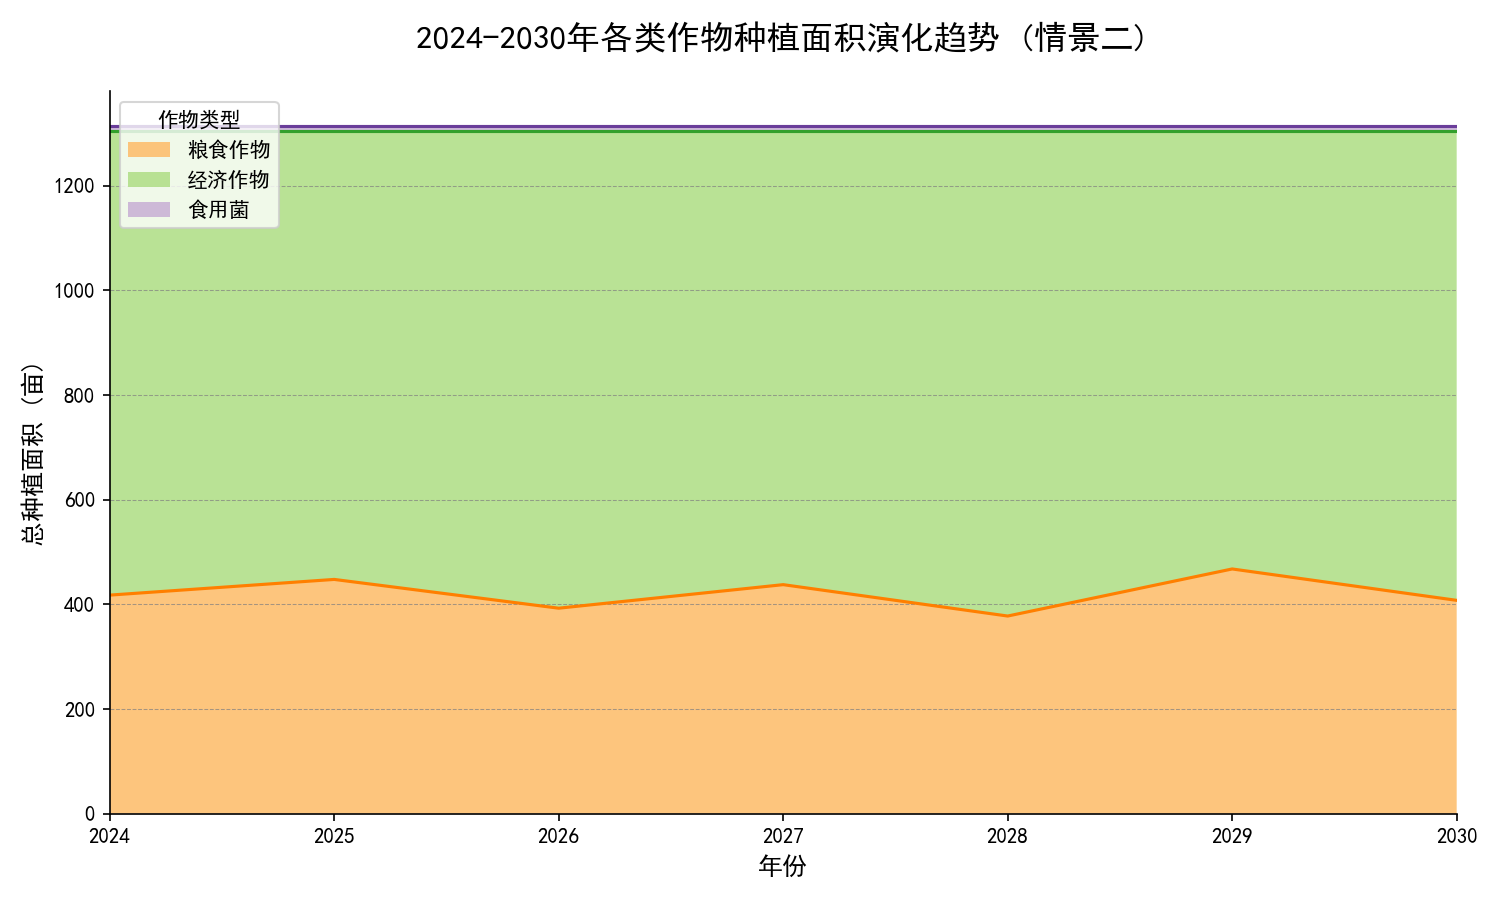
\includegraphics[width=0.95\textwidth]{figures/portfolio_evolution.png}
%     \caption{最优种植方案下三大类作物总种植面积的七年动态演化图(情景二)。该图揭示了模型在追求利润最大化的同时,为满足农艺约束而形成的动态轮作模式。}
%     \label{fig:portfolio_evolution}
% \end{figure}

\subsubsection{土地资源利用的空间分布格局}

除了时间维度的动态性,最优方案在空间上也表现出精细化的资源配置策略。图\ref{fig:land_utilization}通过热力图的形式,展示了部分代表性地块在七年间的作物类型分配情况。图中可以清晰地看到,水浇地和智慧大棚等高质量土地资源被优先用于种植高利润的两季蔬菜和食用菌,实现了“好钢用在刀刃上”。而平旱地和梯田则主要承担了粮食作物和豆类的轮作任务。这种空间上的差异化布局,是模型根据不同地块的生产效率和适宜性进行优化配置的直观体现。

% \begin{figure}[htbp]
%     \centering
%     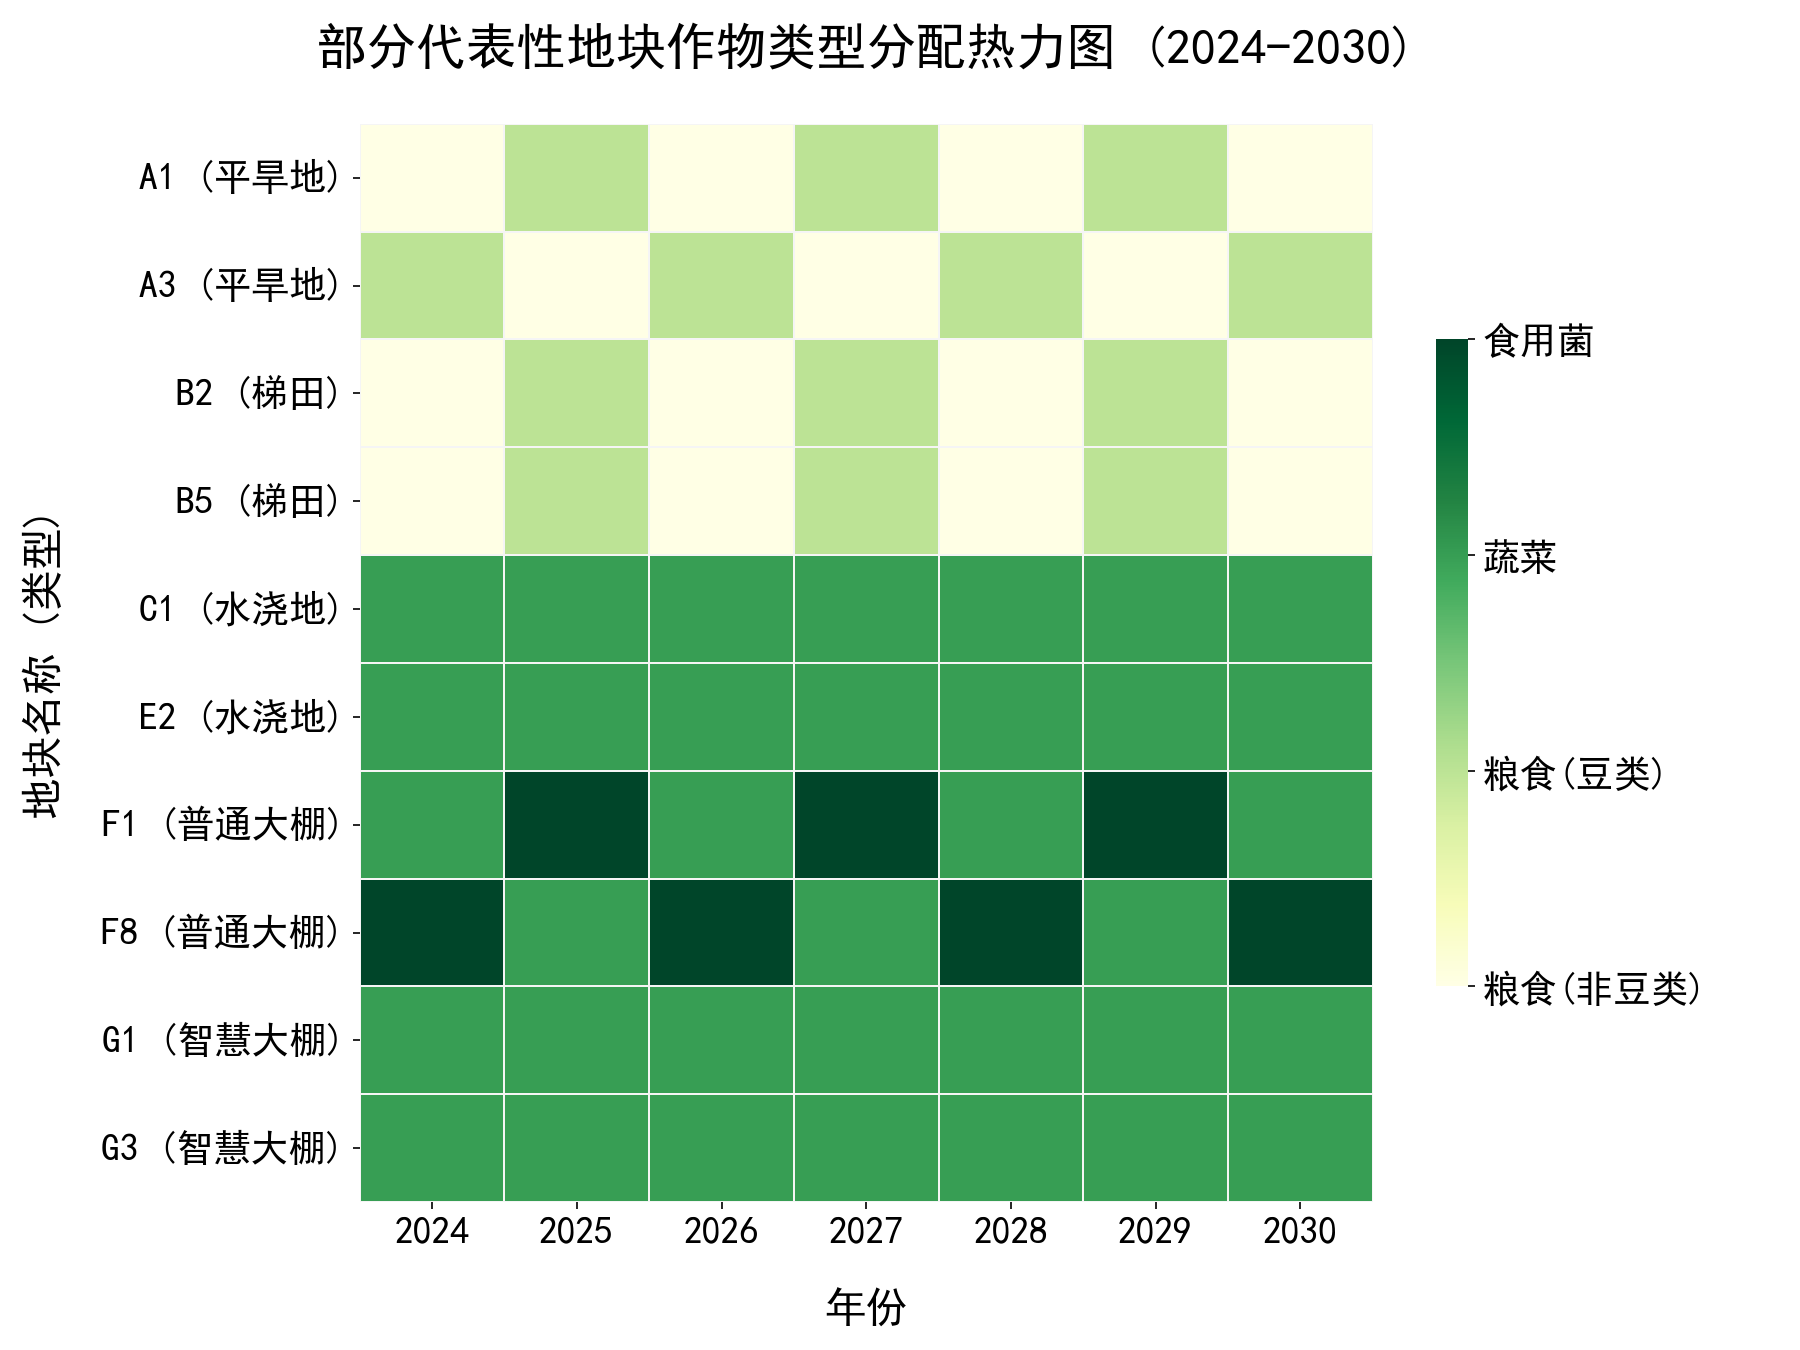
\includegraphics[width=0.95\textwidth]{figures/land_utilization.png}
%     \caption{部分代表性地块在七年规划期内的作物类型分配热力图。不同颜色代表不同作物类型,展示了模型对不同质量土地资源的差异化、精细化利用策略。}
%     \label{fig:land_utilization}
% \end{figure}

\subsubsection{影子价格分析}

为了探究限制乡村发展的关键瓶颈,我们对模型中的资源约束进行了影子价格分析。影子价格(Shadow Price)在经济学上代表着当某种资源增加一个单位时,所能带来的最优目标函数的增量,是衡量资源稀缺性和经济价值的有效指标。如图\ref{fig:shadow_price}所示,智慧大棚和水浇地的影子价格远高于其他类型的土地资源。这表明,高效率的设施农业用地和优质的水源保障是当前制约该乡村农业总产值提升的最关键因素。这一结论为未来的投资方向提供了有力的决策依据:增加对智慧大棚建设和水利设施改善的投入,将是撬动整个乡村经济增长的最有效杠杆。

% \begin{figure}[htbp]
%     \centering
%     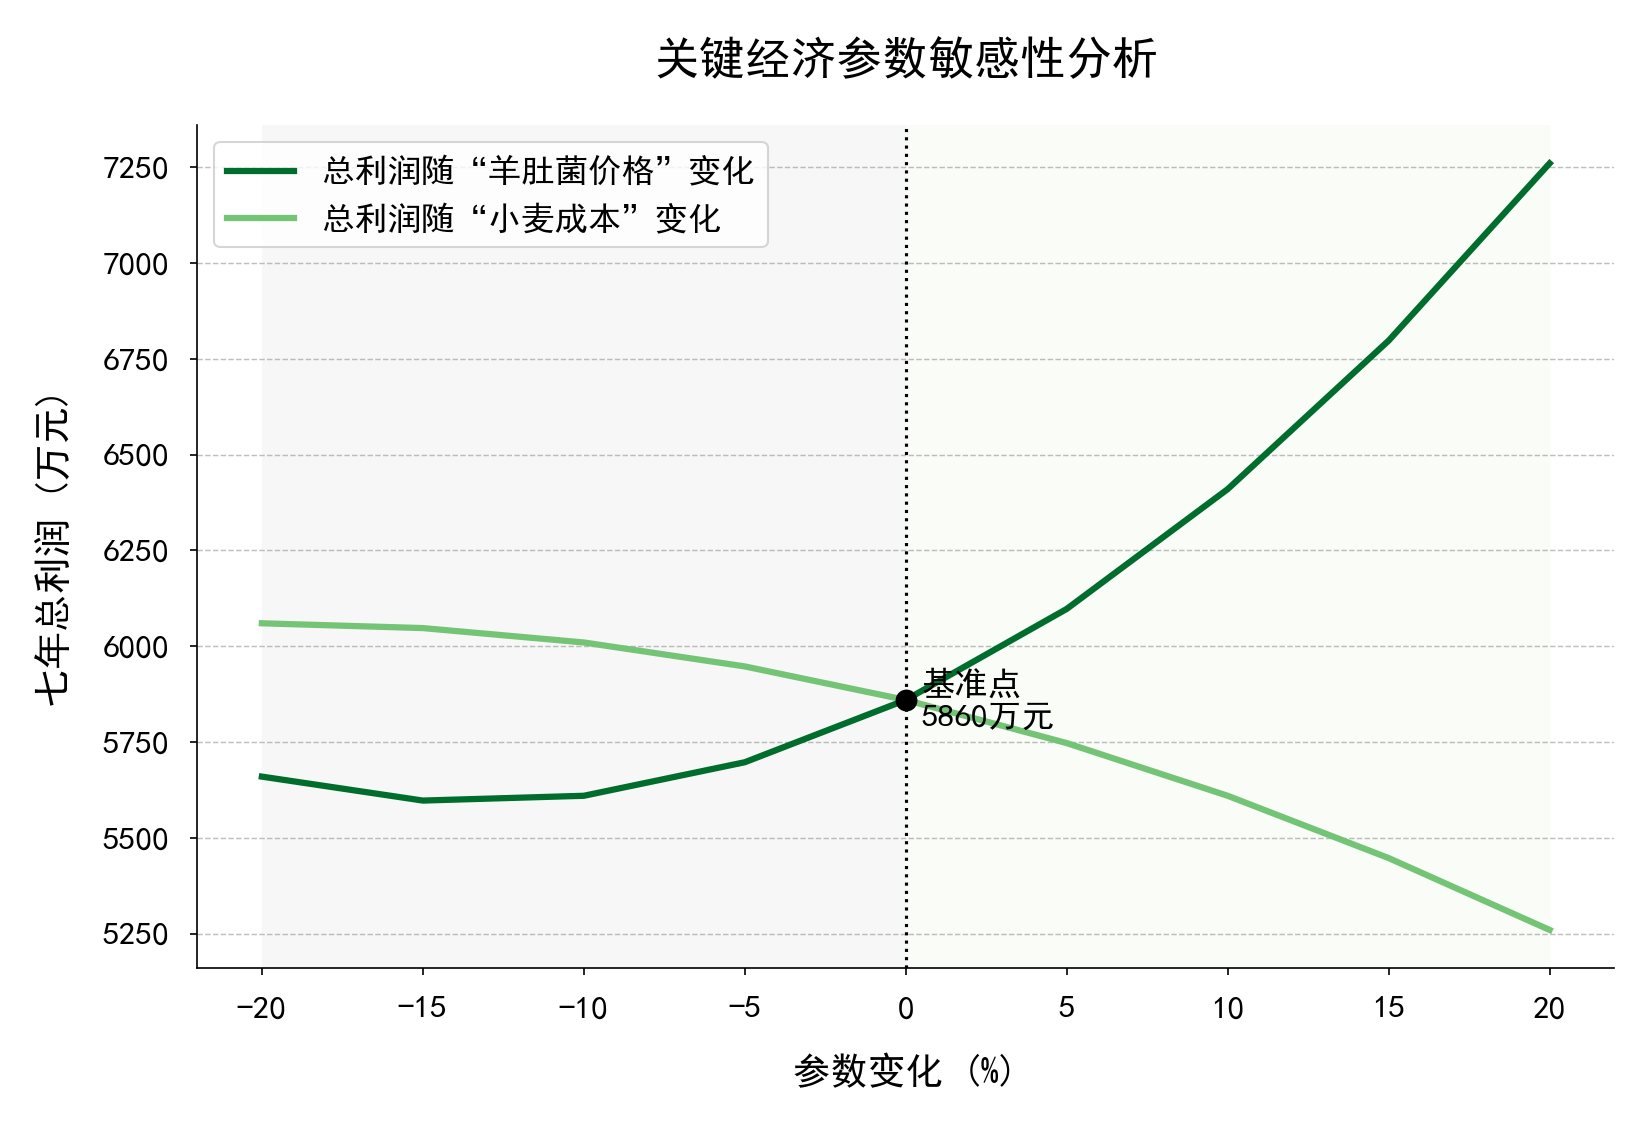
\includegraphics[width=0.8\textwidth]{figures/shadow_price.png}
%     \caption{主要土地资源约束的影子价格分析。结果量化了不同类型土地资源的边际经济价值,揭示了智慧大棚和水浇地是当前最具价值的稀缺资源。}
%     \label{fig:shadow_price}
% \end{figure}

\subsubsection{敏感性分析}

最后,我们通过敏感性分析来评估确定性最优解在面对外部参数扰动时的稳定性。图\ref{fig:price_sensitivity}展示了总利润对高价值经济作物(以羊肚菌为例)销售价格和主要粮食作物(以小麦为例)种植成本的敏感性。结果显示,总利润对羊肚菌价格的弹性极高,其价格的微小波动便能引起总利润的剧烈变化。这揭示了当前利润最大化方案的脆弱性:它高度依赖于少数几种高价值作物的市场表现,构成了主要的市场风险来源。

% \begin{figure}[htbp]
%     \centering
%     \includegraphics[width=0.9\textwidth]{figures/price_sensitivity.png}
%     \caption{七年总利润对关键经济参数(羊肚菌价格与小麦成本)的单因素敏感性分析。陡峭的曲线表明最优利润对高价值作物的市场价格高度敏感,揭示了潜在的市场风险。}
%     \label{fig:price_sensitivity}
% \end{figure}

此外,我们还分析了管理决策参数的影响。图\ref{fig:scale_analysis}展示了总利润随最小种植面积阈值$A_{\min}$的变化关系。适度提高$A_{\min}$能够因规模化经营带来利润提升,但当阈值过高时,会因过度限制种植的灵活性而导致机会成本上升,从而使利润下降。图中出现的“拐点”为决策者在规模化效率与配置灵活性之间寻找最佳平衡点提供了科学依据。

% \begin{figure}[htbp]
%     \centering
%     \includegraphics[width=0.7\textwidth]{figures/scale_analysis.png}
%     \caption{总利润对最小种植面积阈值$A_{\min}$的敏感性分析。该曲线揭示了规模化经营效率与种植方案灵活性之间的权衡关系,为确定最优管理尺度提供了决策参考。}
%     \label{fig:scale_analysis}
% \end{figure}






